\documentclass[a4paper,12pt]{article}
\parindent 0pt
\parskip 1mm
\usepackage{amsmath}
\usepackage[dvips]{epsfig}

\begin{document}

\begin{center}

{\Large\bf CN 510 - Principles and Methods of Cognitive and Neural Modeling}

\bigskip

{\large\bf Assignment \# 9}
\smallskip

{\large\bf John Joseph}
\end{center}

\bigskip
{\bf Correlated Inputs in a Spiking Network}
\bigskip

This assignment is also long overdue, but it is built off of the previous assignments 6 and 8. Rather than generate 100 Poisson spike trains, we are asked to generate 10 and then ``jitter'' those 10 using values taken at random from a Gaussian distribution of $\sigma=3$ milliseconds. We are also, as far as I can tell, told to leave our initial weights alone, though they are still selected at random from a uniform distribution. 

\vspace{2mm}

Another key difference is the fact that we must pipe our pre-synaptic neurons into 20 post-synaptic neurons, rather than one. For this assignment I essentially modified my code from Assignment 8 as follows: I turned off the updating of weights, and I changed my post-synaptic neuron into an array of 20 post-synaptic neurons. 

\vspace{2mm}

I introduced my Gaussian Jitter following the Box-Muller Transformation:

\begin{equation}
R = \sigma \sqrt{-2ln(U)}cos(2\pi V)
\end{equation}

Where U and V are random numbers from the uniform distribution. Once we have generated our 10 poisson trains, we replicate them 9 times each time adding a random jitter value to the pre-existing spike time. The result is a poisson spike train with gaussian jitter. 

\vspace{2mm}

The network consists of 100 pre-synatpic cells all piping into one post-synaptic cell. Based on the input voltage to that cell we generate spikes, and the correlation between the post-synaptic and pre-synaptic spikes will improve or depeciate the bond between those two cells. As such, we have 100 bonds each given some initial weight, and our simulation causes them to spike randomly and see which ones generated the spike that pushed our post-synaptic cell over its threshold.

\vfil\eject

\bigskip
{\bf Synaptic Traces}
\bigskip

I generated my synaptic traces in the same way I did in Assignment 8, stepping through time using boolean values to represent the presence or absence of a spike at any given time. I solved for the spikes using the Rotter-Deissmann method using a C value of 0.5, a remnant of Assignment 8. 

\vspace{2mm}

As with the previous assignment (which I have only just completed...) I am still unable to intregrate the cumulative trace in one go. As such I summed up all pre-synaptic traces into a variable and used that in my post-synaptic integration. Bear in mind, however, that we now have 20 post-synaptic cells, each with it's own unique weight to our 100 pre-synaptic neurons (for a total of 2000 weight values). As such there are 20 individual cumulative values that must be calculated for each post-synaptic neuron. 

\bigskip
{\bf Post-Synaptic Cells}
\bigskip

As I have mentioned, one of the main differences in this week's assignment as opposed to the last is that we now have 20 post-synaptic cells to deal with. Since each has its own bond to all 100 pre-synaptic cells, we must now solve for xCum 20 times for each post-synaptic neuron. We then integrate 20 post-synaptic voltages for these neurons, ensuring we use the correct cumulative values in our calculation. 

\vspace{2mm}

We must also include an inhibitory term in our calculation to simulate competition between post-synaptic cells; this is done using our post-synaptic trace. The trace calculation is identical to what we did in Assignment 8, save for the fact that we do it 20 times. Once we have it, we use it as follows: for the integral of each neuron's post-synaptic potential, we subtract the trace of all other post-synaptic neurons from the cumulative pre-synaptic trace coming in. 

\bigskip
{\bf Discussion}
\bigskip

This assignment was plagued with similar problems to the last one, but the most significant was the inability to keep my post-synaptic voltage in check. I played with four threshold values before deciding on 850v, which is still a very high number. I have plotted this voltage as well as the post-synaptic trace plots for three other threshold values: 400V, 700V and 1000V. 

\vspace{2mm}


The inhibitory nature of the post-synaptic network seemed to play a more noticeable role at higher threshold voltages, where neurons with more favorable spike timings managed to reach the peaks that other neurons could not. Since I chose a value of $C=0.5$ I think this helped in allowing the neurons to play off one another, and trying it with a $C$ value of 1 may yield more stable results. 

\vspace{2mm}

This inhibitory nature probably should have made itself most known in the post-synaptic potential plots, but these were also very threshold-voltage dependent. In general I found that while in the case of a high threshold voltage only certain neurons could cross the threshold, the post-synaptic neurons on average resembled each other quite closely. Any small differences could most likely be attributed to the weight distribution, and this may be one of the crucial things in determining whether or not a post-synaptic neuron live till one of the higher-threshold plots. 

\vspace{2mm}

I would have liked to see more competition between neurons, but I still think my incorrect integration of the post-synaptic voltage is playing a huge part in the error in my results. My code for this calculation is as follows:

\begin{verbatim}
inhib=0;
for (i=0;i<20;i++)
   if (i!=j) inhib+=post[i].x;

V[j] = solveRD(V[j],D,(xCum[j]-inhib)*
     tau*(solveRD(1,D,0)-solveRD(1,A,0)));
\end{verbatim}

For every $j^{th}$ neuron. 

\vspace{2mm}

In particular I would have expected the inhibitory term to significantly reduce the voltage of some neurons, although I suppose my unusually high values would mitigate this impact. 

\vfil\eject 
{\bf Results}
\bigskip

Here are my results, which show the traces of pre-synaptic and post-synaptic neurons as well as the cumulative traces and integrated voltages. However, we start with the rastergram, showing the spike timings of all 100 neurons. THe 100 original Poisson neurons are at the bottom in black, and all other colors represent individual groups of 10 with their own jitter. Note the patterns running up vertically. 

\begin{center}
\begin{figure}[ht!]
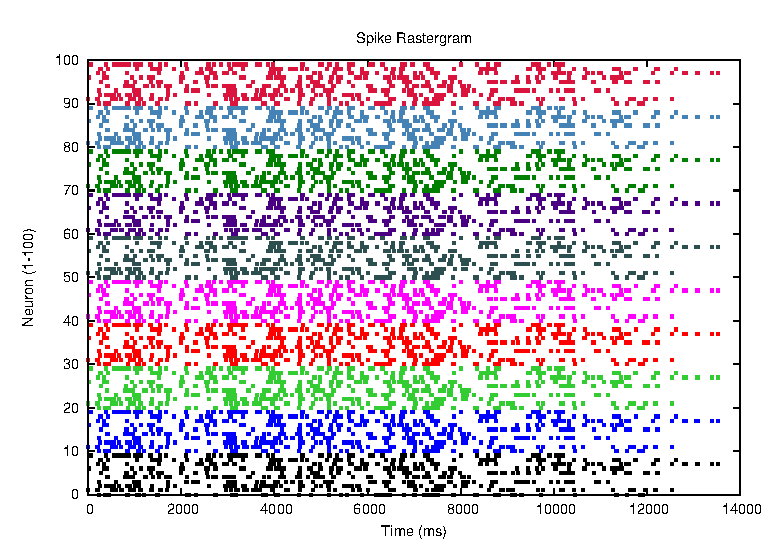
\epsfig{file=data/figures/rasterGram,width=13cm,height=10cm}
\end{figure}
\end{center}

My presynaptic traces were what I had expected, and most of the code I've ported over appears to still be correct. The plot below shows two pre-synapic neurons. 

\vspace{2mm}

My cumulative traces don't tell a huge story, though I think that holding the weight constant allowed that plot to preserve the overall shape of the spikes that went into it. 

\begin{center}
\begin{figure}[ht!]
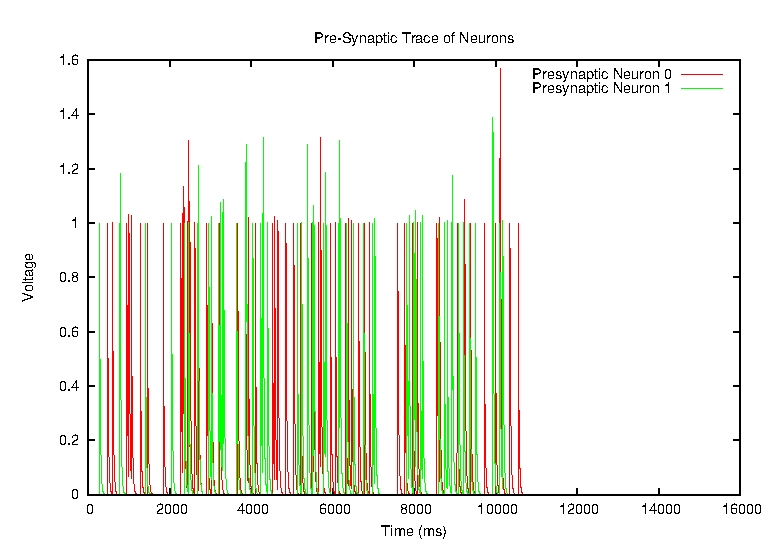
\epsfig{file=data/figures/trace,width=13cm,height=10cm}
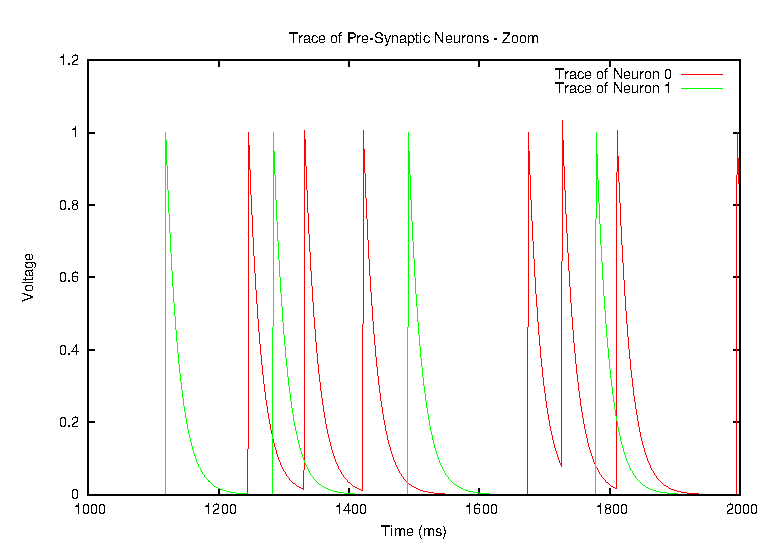
\epsfig{file=data/figures/trace_zoom,width=13cm,height=10cm}
\end{figure}
\end{center}

\begin{center}
\begin{figure}[ht!]
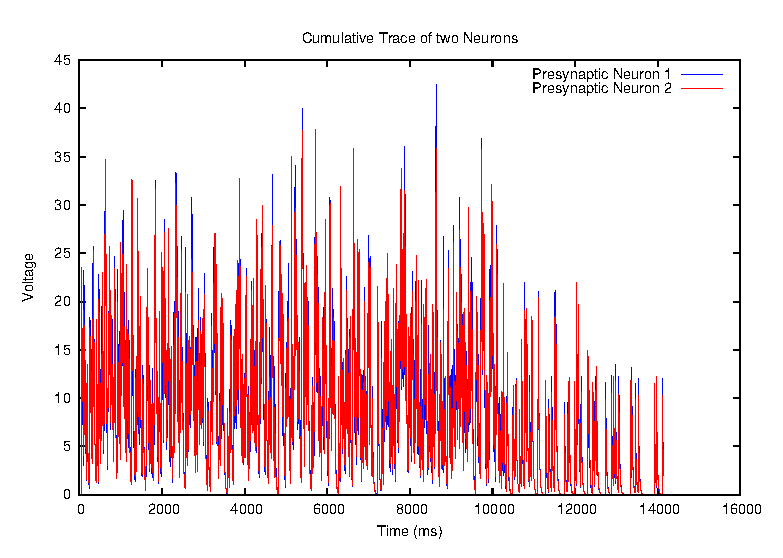
\epsfig{file=data/figures/cumTrace,width=13cm,height=10cm}
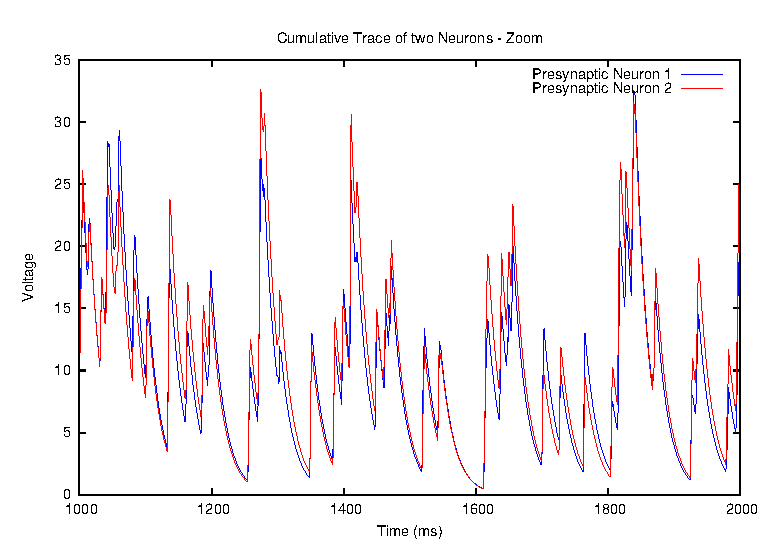
\epsfig{file=data/figures/cumTrace_zoom,width=13cm,height=10cm}
\end{figure}
\end{center}

\begin{center}
\begin{figure}[ht!]
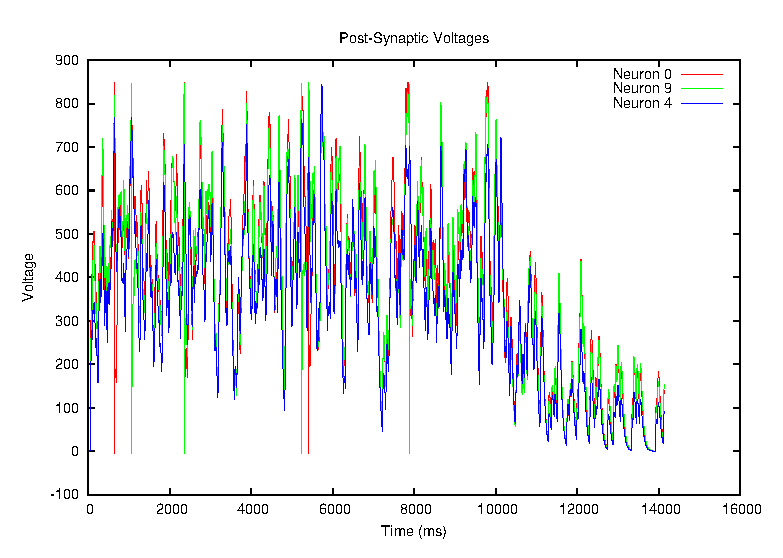
\epsfig{file=data/figures/psp,width=13cm,height=10cm}
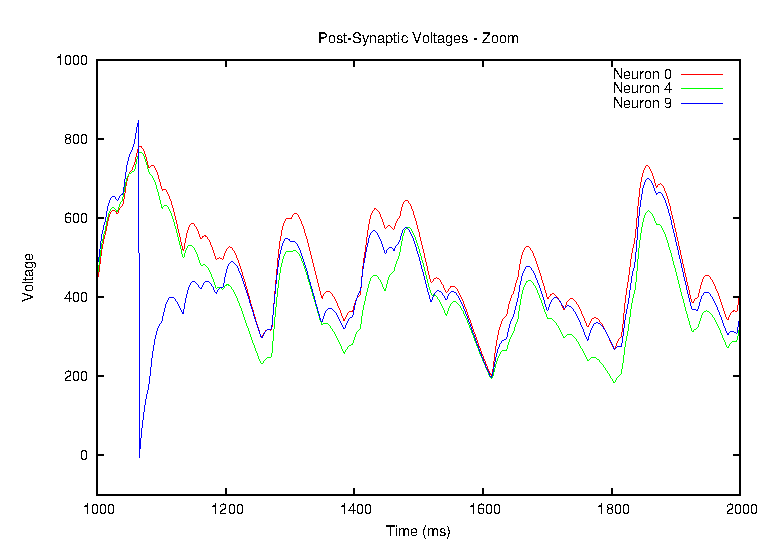
\epsfig{file=data/figures/psp_zoom,width=13cm,height=10cm}
\end{figure}
\end{center}

\begin{center}
\begin{figure}[ht!]
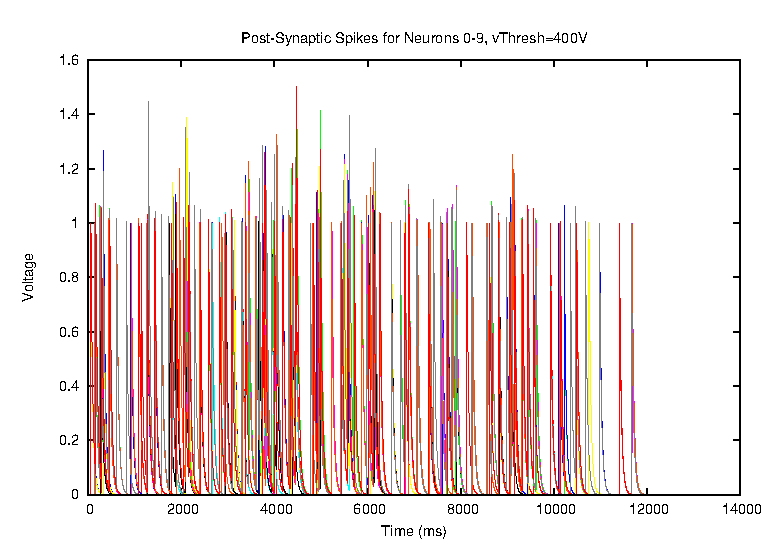
\epsfig{file=data/figures/psp1_9_400,width=13cm,height=10cm}
\end{figure}
\end{center}

The traces of the post-synaptic voltages show how high they were able to get. In those plots I was using a threshold voltage of 850 neurons, and in general all of the post-synaptic potentials were able to reach this height. 

\vspace{2mm}

Above and below are my plots of the post-synaptic spikes for nine neurons at different threshold voltages. Note that while they start out very dense, they start to thin out rapidly. Also note that many of the spikes in the higher threshold plots are overlapped across different post-synaptic neurons. 

\vspace{2mm}

I clearly have a lot of work to do before these plots look correct, and there is is still a lot going wrong here. I hope to fix all of this as soon as possible, as I think they results from these assignments will be very important to the next one. 

\begin{center}
\begin{figure}[ht!]
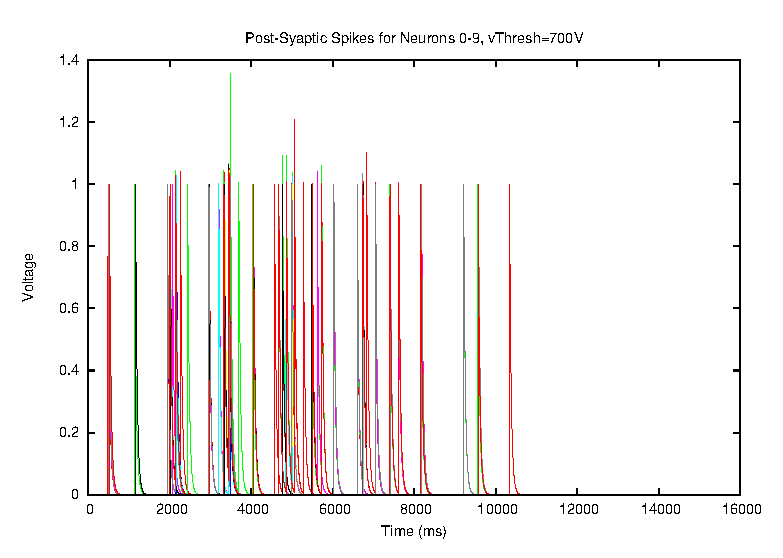
\epsfig{file=data/figures/psp1_9_700,width=13cm,height=10cm}
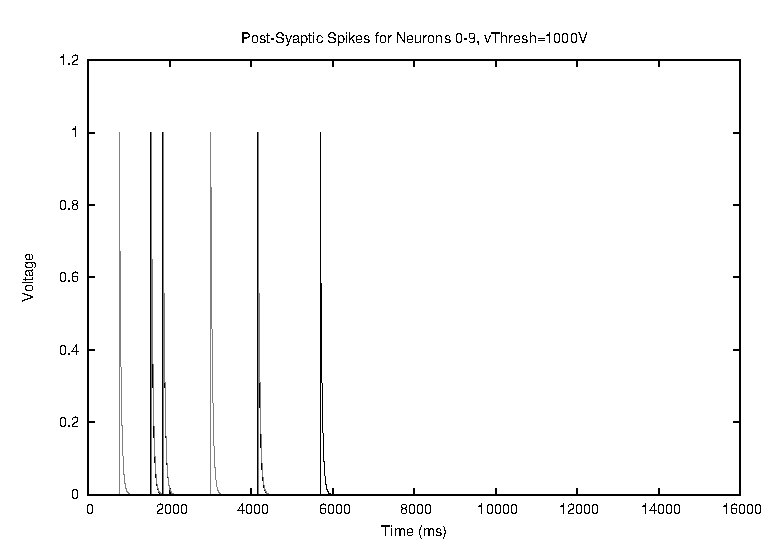
\epsfig{file=data/figures/psp1_9_1000,width=13cm,height=10cm}
\end{figure}
\end{center}

\end{document}
